\chapter{Results} \label{chap:results}

The results of the statistical analysis support the hypotheses outlined in Chapter \ref{chap:contribution} and demonstrate that:
\begin{enumerate}
    \item The effectiveness of requirements crowdsourcing changes with stakeholder network structure.
    \item Crowdsourcing requirements faces diminishing marginal returns, meaning that additional crowdsourcing is less effective for projects that already source a large proportion of requirements from the crowd
    \item More concentrated stakeholder networks are associated with stronger project management outcomes
\end{enumerate}

In addition to showing that stakeholder network structure impacts OSS project performance, the results indicate that the effect changes depending on the current share of crowdsourced requirements. More concentrated stakeholder networks---and specifically those with a hub-and-spoke structure---coincide with better outcomes for requirement close-out and response times and comment activity. The analysis shows that requirements crowdsourcing faces diminishing marginal returns. Once OSS projects crowdsource more than 70\% of requirements, they face slower close-out and response times, a backlog of unaddressed requirements, and worse crowd retention. This suggests that, beyond that point, OSS project managers should focus on using CrowdRE techniques to organize and prioritize existing requirements rather than incentivizing the crowd to generate additional requirements. These results only apply to active OSS projects, and may not generalize well to other scenarios, including OSS projects in the design phase, proprietary software projects, or physical products such as hardware. Additionally, crowds in this data set have relatively high levels of software development expertise, limiting the applicability of this study to less technically adept crowds. Before covering the regression results in detail, this section will provide an overview of the output of the stakeholder network generation process.

An implication of these results is that OSS project managers should employ different CrowdRE techniques depending on the specific circumstances for their project. For projects that currently source a limited share of requirements from the crowd, project managers should use techniques such as gamification~\cite{dalpiaz} and micro-crowds~\cite{levy} to encourage additional crowd participation. Micro-crowds also have the benefit of promoting stakeholder networks with a hub-and-spoke structure, which have stronger project management outcome. As the share of crowdsourced requirements rises, OSS project manager should transition to  CrowdRE strategies for efficiently triaging and prioritizing existing requirements, such as automated recommender systems~\cite{mobasher}.

\section{Stakeholder Networks}

For each of the 562 projects in the data set, this study used automated code to generate the stakeholder networks using the method described in Section \ref{network_section} and calculate the network metrics using the method described in Section \ref{network_structure}. Network structure diagrams for four of the projects appear in Figure \ref{network_plots}. From left to right and top to bottom, these diagrams depict the stakeholder networks for the Amazon Web Service software development kit for PHP, the tmux terminal multiplexer, the KeystoneJS JavaScript content manager, and Derive4J, a pattern matching tool for Java. Each of these open-source tools has wide adoption and a broad user base. Nevertheless, their network structures vary considerably. The full data set contains an even more extensive range of network configurations.

\begin{figure*}
  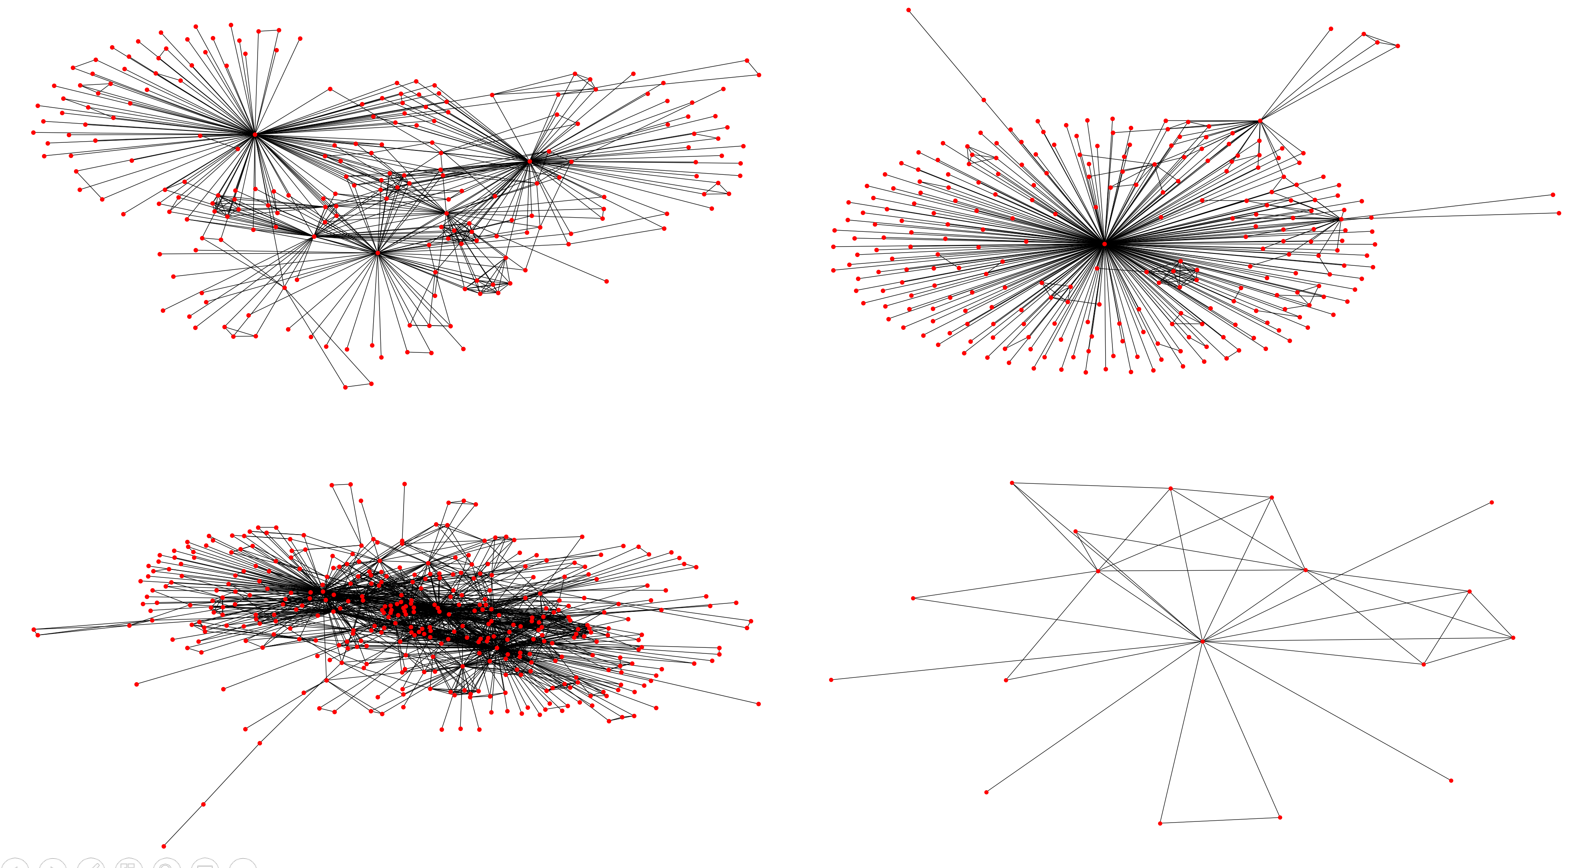
\includegraphics[width=.95\textwidth]{img/network_plots.PNG}
\caption{Example network plots}
\label{network_plots}
\end{figure*}

Table \ref{network_summary} shows the summary statistics for each of the network structure variables. For the Gini coefficient, the summary statistics show a tight cluster of stakeholder networks with a moderate level of concentration, contrasted with a smaller number of highly- and lowly-concentrated networks on either end of the distribution. The statistics for average minimum path indicate that most of the stakeholder networks are, per Watts and Strogatz~\cite{watts}, relatively small-worlds, although the data set does show substantial variability in the breadth of the networks. The clustering coefficient takes on the most diverse distribution of values, ranging from networks with virtually no localized clustering, such as the network for tmux in Figure \ref{network_structure}, to highly integrated networks, such as the network for KeystoneJS.

\begin{table}
\caption{Summary Statistics for Network Variables}
\label{network_summary}
\begin{tabular}{llllll}
\hline\noalign{\smallskip}
Variable & Min & 25\% & Median & 75\% & Max  \\
\noalign{\smallskip}\hline\noalign{\smallskip}
Gini Coeff. & 0.29 & 0.54 & 0.57 & 0.59 & 0.70 \\
Avg. Min. Path & 1.40 & 2.01 & 2.15 & 2.33 & 3.05 \\
Clustering Coeff. & 0.00 & 0.52 & 0.63 & 0.70 & 0.88 \\
\noalign{\smallskip}\hline
\end{tabular}
\end{table}

The scatter plots in Figures \ref{crowd_pct_gini_plot}, \ref{crowd_pct_avg_min_path_plot}, and \ref{crowd_pct_clustering_plot} show that crowdsourcing occurs at varying intensities across all network types. The wide distribution of crowdsourcing intensities across network structures also makes statistical inference more reliable. Specifically, the distribution allows the models to capture how crowdsourcing interacts with network structure without having to worry about (a) combinations of crowdsourcing and network structure that fall outside the range of observed values in the data set and (b) excessive collinearity between the covariates. This property makes the data set ideal for assessing how network structure impacts the effectiveness of CrowdRE.

\begin{figure*}
 \includegraphics[width=.85\textwidth]{img2/crowd_pct_vs_gini_coefficient.png}
\caption{Share of Crowdsourced Requirements vs. Gini Coefficient}
\label{crowd_pct_gini_plot}
\end{figure*}

\begin{figure*}
 \includegraphics[width=.85\textwidth]{img2/crowd_pct_vs_avg_min_path.png}
\caption{Share of Crowdsourced Requirements vs. Avg. Min Path}
\label{crowd_pct_avg_min_path_plot}
\end{figure*}

\begin{figure*}
 \includegraphics[width=.85\textwidth]{img2/crowd_pct_vs_clustering.png}
\caption{Share of Crowdsourced Requirements vs. Clustering Coefficient}
\label{crowd_pct_clustering_plot}
\end{figure*}

\section{Regression Results}

\subsection{Requirement Close-Out Time}

Within the data set, the average number of days a requirement remains active ranges from less than a day to several years. On average, most projects closeout requirements within three months, although the data set does included several projects with very long average close-out times. The results of a KS test fail to reject the null hypothesis that close-out time follows a Gamma distribution, making the Gamma GLM a reasonable model choice.

\begin{figure*}
  \includegraphics[width=.85\textwidth]{img2/active_time_hist.png}
\caption{Active Time Histogram}
\label{active_time_hist}
\end{figure*}

\begin{figure*}
  \includegraphics[width=.85\textwidth]{img2/active_time_resid.png}
\caption{Active Time Residuals}
\label{active_time_resid}
\end{figure*}

\begin{figure*}
  \includegraphics[width=.85\textwidth]{img2/active_time_resid_hist.png}
\caption{Active Time Residuals Histogram}
\label{active_time_resid_hist}
\end{figure*}

Table \ref{active_time_regression} shows the regression results. All seven variables are statistically significant. The residual plot in Figure \ref{active_time_resid} shows no relationship between requirement close-out time and the residuals, which means the results do not raise any concerns about biased estimators.

\begin{table}
\caption{Regression on Requirement Close-Out Time}
\label{active_time_regression}
\begin{tabular}{lll}
Gamma GLM | Pseudo $R^2$: 0.51 \\
\hline\noalign{\smallskip}
Variable & Coefficient & p-value  \\
\noalign{\smallskip}\hline\noalign{\smallskip}
Intercept & 0.98 & 0.05 \\
Crowd Percentage & 4.36 & $\leq 0.01$  \\
Avg Min Path & 0.75 & $\leq 0.01$ \\
Clustering x Crowd Percentage & 3.06 & $\leq 0.01$ \\
Avg Min Path x Crowd Percentage & -1.29 & $\leq 0.01$ \\
Gini Coefficient x Crowd Percentage & -4.75 & $\leq 0.01$ \\
Project Age & 0.0005 & $\leq 0.01$ \\
Nodes & 0.0004 & $\leq 0.01$ \\
\noalign{\smallskip}\hline
\end{tabular}
\end{table}

\begin{figure*}
  \includegraphics[width=0.85\textwidth]{img2/active_time_marginal_avg_min_path.png}
\caption{Close-Out Time Marginal - Average Min Path}
\label{active_time_marginal_avg_min_path}
\end{figure*}

\begin{figure*}
  \includegraphics[width=0.85\textwidth]{img2/active_time_marginal_clustering.png}
\caption{Close-Out Time Marginal - Clustering Coefficient}
\label{active_time_marginal_clustering}
\end{figure*}

\begin{figure*}
  \includegraphics[width=0.85\textwidth]{img2/active_time_marginal_gini.png}
\caption{Close-Out Time Marginal - Gini Coefficient}
\label{active_time_marginal_gini}
\end{figure*}

Figures \ref{active_time_marginal_avg_min_path}, \ref{active_time_marginal_clustering}, and \ref{active_time_marginal_gini} show how the marginal effect of increasing the proportion of crowdsourced requirements changes with network structure. For dispersed networks with high concentration and low levels of localized clustering, increasing the share of crowdsourced requirements does not result in substantial increases in requirement close-out time. Networks with the opposite characteristics suffer accelerating requirement close-out times as the share of crowdsourced requirements increases, which indicates that project teams cannot keep up with a growing backlog of crowdsourced requirements. Figure \ref{reqs_contributors_over_time} shows how the total volume of outstanding requirements grows more quickly than the total number of contributors working on the projects. While the figure shows two example projects---KeystoneJS and LeafletJS---the trend holds broadly across the data set. These results point to stakeholder networks with well-defined hubs as a more effective configuration for OSS projects. These results confirm the hypothesis in Chapter \ref{chap:contribution}, which expects requirement close-out time to rise as the share of crowdsourced requirements increases. The results also validate conclusions from Iyer and Lyytinen~\cite{iyer} and Toral, et al.~\cite{toral} which find that more concentrated stakeholder networks have higher task completion rates.

\begin{figure*}
  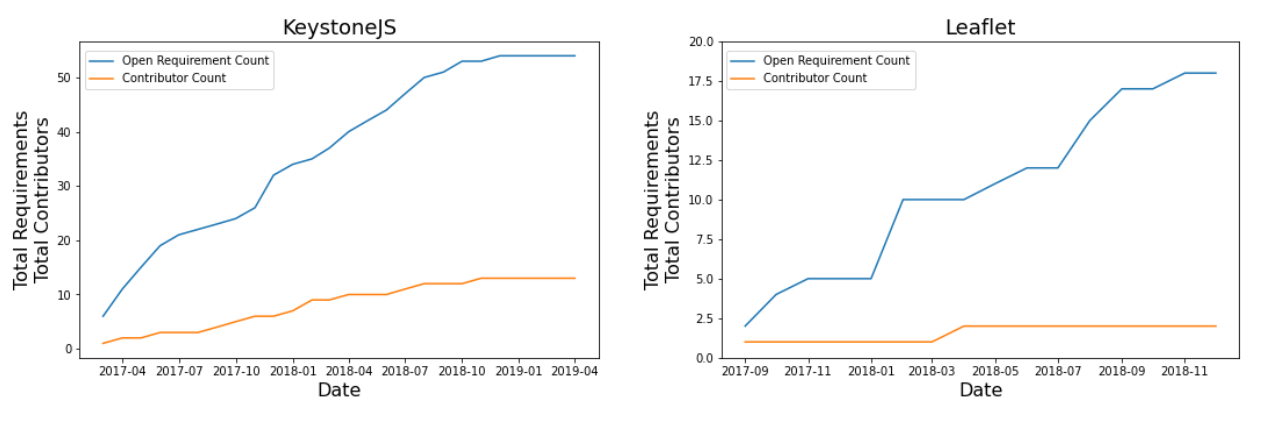
\includegraphics[width=0.95\textwidth]{img/reqs_contributors_over_time.PNG}
\caption{Open requirements compared to code contributors over time}
\label{reqs_contributors_over_time}
\end{figure*}

\subsection{Requirement Response Time}

The average response times in the data set range from within a day to slightly over a year. As the histogram in Figures \ref{response_time_hist} shows, the observations follow a lifetime distribution with a long right tail. On average, most projects teams respond to requirements within a month.

\begin{figure*}
  \includegraphics[width=0.85\textwidth]{img2/response_time_hist.png}
\caption{Response Time Histogram}
\label{response_time_hist}
\end{figure*}

\begin{figure*}
  \includegraphics[width=0.85\textwidth]{img2/response_time_resids.png}
\caption{Response Time Residuals}
\label{response_time_resids}
\end{figure*}

\begin{figure*}
  \includegraphics[width=0.85\textwidth]{img2/response_time_resids_hist.png}
\caption{Response Time Residuals Histogram}
\label{response_time_resids_results}
\end{figure*}

Table \ref{reaction_time_regression} shows the regression results for requirement response time. For response time, the OLS model had an adjusted $R^2$ of 0.56 compared to a pseudo-$R^2$ of 0.43 for the Gamma GLM. Due to better model performance and because the model appeared to conform to the Gauss-Markov assumptions, the OLS model is more appropriate in this scenario. The OLS model includes eight variables, all of which demonstrate statistical significance. As shown in Figure \ref{response_time_resids}, the residuals approximate a normal distribution and do not correlate with the response variable. Therefore, the model adheres to the Gauss-Markov assumptions and does not appear likely to suffer from biased estimators.

\begin{table}
\caption{Regression on Response Time}
\label{reaction_time_regression}
\begin{tabular}{lll}
OLS Regression | $R^2$: 0.57 | Adjusted $R^2$: 0.56 \\
\hline\noalign{\smallskip}
Variable & Coefficient & p-value  \\
\noalign{\smallskip}\hline\noalign{\smallskip}
Crowd Percentage Squared & 72.48 & $\leq 0.01$ \\
Gini Coefficient & -69.34 & 0.03 \\
Gini Coefficient X Crowd Percentage & -273.75 & $\leq 0.01$ \\
Clustering Coefficient & -50.78 & 0.03 \\
Clustering Coefficient x Crowd Percentage & 148.08 & $\leq 0.01$ \\
Avg Min Path & 34.13 & $\leq 0.01$ \\
Project Age & 0.02 & $\leq 0.01$ \\
\noalign{\smallskip}\hline
\end{tabular}
\end{table}

The marginal effect plots in Figures \ref{response_time_marginal_total}, \ref{response_time_marginal_clustering}, and \ref{response_time_marginal_gini} demonstrate that the impact of requirements crowdsourcing changes dramatically with the structure of the networks. Whereas crowdsourcing a greater share of requirements reduces reaction time for networks with high concentration and low localized clustering, the opposite holds for networks with high localized clustering and low concentration. The direction changes where the marginal effect curves cross zero, switching from negative to positive in the marginal effects plots noted above. Networks with faster response times have a hub-and-spoke structure, suggesting stronger performance for more concentrated stakeholder networks. Moreover, the results show that the marginal impact on response time increases with the share of crowdsourced requirements in the OSS project, which implies that requirements crowdsourcing faces decreasing marginal returns. 

Overall, these results suggest that OSS project may benefit from either an automated system for prioritizing requirements or a community manager responsible for managing and assigning requirements. These observations reinforce existing results~\cite{stakesource, stakerare, lim, mobasher} within the collaborative requirements elicitation literature, which suggest the use of stakeholder network mapping or automated recommender systems to help manage requirements. The results for requirement response time provide evidence in support of the hypotheses that requirements crowdsourcing faces diminishing marginal returns. The negative correlation between the Gini coefficient and the response time also bolsters the hypothesis that more concentrated stakeholder networks have more favorable project management outcomes. Finally, the results confirm the specific prediction that an increase in the share of crowdsourced requirements lengthens the average response time.

\begin{figure*}
  \includegraphics[width=0.85\textwidth]{img2/response_time_marginal_total.png}
\caption{Response Time Marginal - Total}
\label{response_time_marginal_total}
\end{figure*}

\begin{figure*}
  \includegraphics[width=0.85\textwidth]{img2/response_time_marginal_avg_clustering.png}
\caption{Response Time Marginal - Clustering Coefficient}
\label{response_time_marginal_clustering}
\end{figure*}

\begin{figure*}
  \includegraphics[width=0.85\textwidth]{img2/response_time_marginal_gini.png}
\caption{Response Time Marginal - Gini Coefficient}
\label{response_time_marginal_gini}
\end{figure*}

\subsection{Comment Activity}
\label{comment_activity}

As noted in Section \ref{measures_of_effectiveness}, average comment activity indicates stronger engagement in the requirements formation process~\cite{toral}. Therefore, higher average comment activity represents a positive outcome. Figure \ref{comment_activity_hist} includes a histogram showing the distribution of average comments within the data set. The histogram shows that average comment activity has an approximately normal distribution and ranges from 1-8 comments per requirement. While the histogram for comment activity appears normal, since it has a positive domain, modeling comment activity with a Gamma distribution remains a reasonable choice. Since the Gamma distribution constitutes a sum of Exponential random variables, the Central Limit Theorem implies that a Gamma distribution can approximate a normal distribution if parameterized properly~\cite{wackerly}. Indeed, the results of the KS tests show that the comment activity data fit both the normal and Gamma distributions well under their maximum likelihood estimates. Under these conditions, either a Gamma GLM or an OLS model are sensible options. In this case, the Gamma GLM is preferable due to materially better model performance.

\begin{figure*}
 \includegraphics[width=0.85\textwidth]{img2/comment_activity_hist.png}
\caption{Comment Activity Histogram}
\label{comment_activity_hist}
\end{figure*}

\begin{figure*}
 \includegraphics[width=0.85\textwidth]{img2/comment_activity_resid.png}
\caption{Comment Activity Residuals}
\label{comment_activity_resid}
\end{figure*}

\begin{figure*}
 \includegraphics[width=0.85\textwidth]{img2/comment_activity_resid_hist.png}
\caption{Comment Activity Residuals Histogram}
\label{comment_activity_resid_hist}
\end{figure*}

Table \ref{comment_activity_regression} presents the regression results. The model contains 21 variables. Each variable in the regression model is statistically significant. Residual plots for the regression appear in Figures \ref{comment_activity_hist}, \ref{comment_activity_resid}, and \ref{comment_activity_resid_hist}. The residual plots show a positive correlation between the residuals and the response variables. However, a linear regression between the dependent variables and the residuals reveals no statistically significant relationship, leading to no concern about biased estimators for this model.

\begin{table}
\caption{Regression on Comment Activity}
\label{comment_activity_regression}
\begin{tabular}{lll}
Gamma GLM | Pseudo $R^2$: 0.46 \\
\hline\noalign{\smallskip}
Variable & Coefficient & p-value  \\
\noalign{\smallskip}\hline\noalign{\smallskip}
Intercept & 0.98 & $\leq 0.01$ \\
Crowd Pct & 4.10 & $\leq 0.01$ \\
Crowd Pct Squared & -3.12 & $\leq 0.01$ \\
Crowd Pct Cubed & 1.69 & $\leq 0.01$ \\
Avg Min Path Squared & 0.35 & $\leq 0.01$ \\
Avg Min Path x Crowd Pct &  -2.37 & $0.02$ \\
Gini Squared & 2.90 & $0.04$ \\
Gini x Avg Min Path & -2.37 & $\leq 0.01$ \\
Gini x Clustering & 5.76 & $\leq 0.01$ \\
Gini x Avg Min Path x Crowd Pct & 3.03 & $\leq 0.01$ \\
Gini x Clustering  x Crowd Pct & -11.24 & $\leq 0.01$ \\
Clustering Squared & 1.68 & $\leq 0.01$ \\
Clustering x Avg Min Path & -1.68 & $\leq 0.01$ \\
Clustering x Avg Min Path x Crowd Pct & 2.12 & $\leq 0.01$ \\
Avg First Comment & -0.002 & $\leq 0.01$ \\
Avg Active Time & 0.001 & $\leq 0.01$ \\
\noalign{\smallskip}\hline
\end{tabular}
\end{table}

The share of crowdsourced requirements and the structure of the stakeholder network have a greater effect on comment activity than on any other measure of effectiveness. The overall trend shows that requirements for OSS projects with very low and very high proportions of crowdsourced requirements generate less discussion than requirements for OSS projects with a moderate share of crowdsourced requirements. Generally, less locally clustered and less concentrated networks generate more comment activity, although the difference for network concentration diminishes for OSS projects with higher proportions of crowdsourced requirements. For dispersed networks, the marginal effect on comment activity remains relatively flat at all levels of crowdsourcing, while networks with a lower average minimum path experience a more pronounced decrease at moderate ranges. Since networks with less localized clustering perform better with respect to comment activity and concentration has a limited effect, these results remain consistent with the hypothesis that stakeholder networks with multiple hubs foster more effective crowd participation in the requirements generation process for OSS projects. Moreover, comment activity is the measure of effectiveness that provides the most evidence in favor of the assertion that stakeholder network structure and the share of crowdsourced requirements have a joint effect on project management outcomes, as the results show substantial interaction between the network structure and crowdsourcing variables.

\begin{figure*}
  \includegraphics[width=0.85\textwidth]{img2/comment_activity_marginal_total.png}
\caption{Comment Activity Marginal - Total}
\label{comment_activity_marginal_total}
\end{figure*}

\begin{figure*}
  \includegraphics[width=0.85\textwidth]{img2/comment_activity_marginal_avg_min_path.png}
\caption{Comment Activity Marginal - Avg. Min Path}
\label{comment_activity_marginal_avg_min_path}
\end{figure*}

\begin{figure*}
  \includegraphics[width=0.85\textwidth]{img2/comment_activity_marginal_clustering.png}
\caption{Comment Activity Marginal - Clustering Coef.}
\label{comment_activity_marginal_clustering}
\end{figure*}

\begin{figure*}
  \includegraphics[width=0.85\textwidth]{img2/comment_activity_marginal_gini.png}
\caption{Comment Activity Marginal - Gini Coef.}
\label{comment_activity_marginal_gini}
\end{figure*}

\subsection{Contributor Retention Time}

As with comment activity and requirements per crowd member, contributor retention time reflects strong engagement from the crowd. OSS projects benefit by retaining participants for a longer time. The histogram in Figure \ref{retention_time_hist} shows that most crowd members engage with an OSS project for only a few months, although the distribution has a long tail and many crowd members remain engaged for a longer period of time. A KS test on the data shows that, under the maximum likelihood estimates, the response data conforms to a Gamma distribution, making the Gamma GLM a reasonable choice for the regression model. 

\begin{figure*}
 \includegraphics[width=0.85\textwidth]{img2/retention_time_hist.png}
\caption{Retention Time Histogram}
\label{retention_time_hist}
\end{figure*}

\begin{figure*}
 \includegraphics[width=0.85\textwidth]{img2/comment_activity_resid.png}
\caption{Retention Time Residuals}
\label{retention_time_resid}
\end{figure*}

\begin{figure*}
 \includegraphics[width=0.85\textwidth]{img2/comment_activity_resid_hist.png}
\caption{Retention Time Residuals Histogram}
\label{retention_time_resid_hist}
\end{figure*}

Table \ref{retention_time_results} shows the results for the regression. Each variable demonstrates statistical significance. The residual plots, shown in Table \ref{retention_time_resid}, show no relationship between the response variables and the residuals, meaning biased estimators do not present a serious concern. A regression of the independent variables against the residuals confirms this assessment.

\begin{table}
\caption{Regression on Retention Time}
\label{retention_time_results}
\begin{tabular}{lll}
Gamma GLM | Pseudo $R^2$: 0.42 \\
\hline\noalign{\smallskip}
Variable & Coefficient & p-value  \\
\noalign{\smallskip}\hline\noalign{\smallskip}
Intercept &  4.02 & $\leq 0.01$ \\
Average Min Path x Crowd Percentage &  -1.12 & $\leq 0.01$ \\
Average Close-out Time &  -0.0021 &  $0.03$  \\
Total Open Issues &  0.0011 &  $0.01$    \\
Project Age &  0.0006 &  $\leq 0.01$    \\
Total Project Contributors &  -0.016 &  $\leq 0.01$ \\
\noalign{\smallskip}\hline
\end{tabular}
\end{table}

Of the network structure variables, only average minimum path had an effect on retention time. The impact of average minimum path on average retention time changes with the share of crowdsourced requirements. Table \ref{retention_time_results} shows the marginal effect on average retention time of an increase in the proportion of crowdsourced requirements. Under all conditions, an increasing the share of crowdsourced requirements decreases average retention time, although the magnitude of the effect diminishes once an OSS project crowdsources a higher proportion of requirements. While additional crowdsourcing has a less detrimental effect on OSS projects with less dispersed stakeholder networks, network structure ceases to have a major impact once a project sources more than 40\% of requirements from the crowd. The results of this regression confirm concerns in the CrowdRE literature~\cite{glinz, groen, levy} about maintaining motivation in large crowds and suggests OSS projects could benefit from adopting CrowdRE methods such as gamification. 

\begin{figure*}
  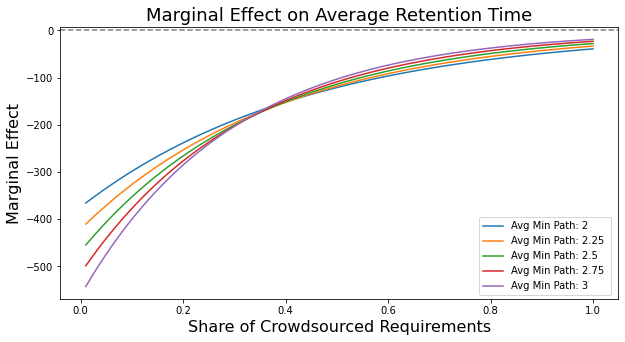
\includegraphics[width=0.85\textwidth]{img2/retention_time_marginal.png}
\caption{Retention Time Marginal - Avg. Min Path}
\label{retention_time_marginal_avg_min_path}
\end{figure*}

\subsection{Requirements Per Crowd Member}

The average number of requirements per crowd member measures the intensity of engagement between the project team and the crowd. Multiple requirement submissions by a single crowd member signals strong engagement and represents a positive outcome for an OSS project. As shown in Figure \ref{issues_per_user_hist}, for most projects, each crowd member submits relatively few requirements. However, the distribution has a long right tail, and some projects average several dozen requirements per crowd member. The results of the KS test validate that the variable conforms to a Gamma distribution, per the assumptions of the Gamma GLM.

\begin{figure*}
  \includegraphics[width=0.85\textwidth]{img2/issues_per_user_hist.png}
\caption{Requirements Per User Histogram}
\label{issues_per_user_hist}
\end{figure*}

\begin{figure*}
  \includegraphics[width=0.85\textwidth]{img2/issues_per_user_resid.png}
\caption{Requirements Per User Residuals}
\label{issues_per_user_resid}
\end{figure*}

\begin{figure*}
  \includegraphics[width=0.85\textwidth]{img2/issues_per_user_resid_hist.png}
\caption{Requirements Per User Residuals Histogram}
\label{issues_per_user_resid_hist}
\end{figure*}


The regression results for the network and requirements crowdsourcing variables appear in Table \ref{issues_per_user_regression}. In contrast to the other measures of effectiveness, the variable selection process only selected a small number of regressors for this model. The model includes three variables, each of which demonstrates statistical significance. Of the network structure variables, only average minimum path appears in the equation. Its effect, however, does not change with the share of crowdsourced requirements. Other network structure variables do not have a statistically significant effect when included in the regression.  This leads to the conclusion that, while the proportion of crowdsourced requirements affects the number of requirements per crowd member, the effect does not change with the structure of the stakeholder network. 


\begin{table}
\caption{Regression on Requirements Per User}
\label{issues_per_user_regression}
\begin{tabular}{lll}
Gamma GLM | Pseudo $R^2$: 0.64 \\
\hline\noalign{\smallskip}
Variable & Coefficient & p-value  \\
\noalign{\smallskip}\hline\noalign{\smallskip}
Intercept & 2.17 & $\leq 0.01$ \\
Crowd Percentage & -7.90 & $\leq 0.01$ \\
Crowd Percentage Squared & 6.40 & $\leq 0.01$  \\
Avg Min Path & 0.52 & $\leq 0.01$  \\
\noalign{\smallskip}\hline
\end{tabular}
\end{table}

Figure \ref{issues_per_user_resid} shows a positive correlation between requirements per crowd member and the residuals. A linear regression of the residuals against the dependent variables shows a slight positive correlation between crowd percentage and the residuals, and a slight negative correlation between crowd percentage squared and the residuals. These results imply bias toward zero for both of the coefficients, meaning the model probably overestimates the effect of crowdsourcing. However, the base and squared crowdsourcing terms both have roughly the same coefficient in the residual regression, meaning the positive-to-negative crossover point remains unbiased, even though the GLM overestimates the overall effect of crowdsourcing.

The coefficients indicate that additional crowdsourcing decreases the number of requirements per crowd member for projects that source less that 65\% of their requirements from the crowd, and increases the number of requirements per crowd member beyond that threshold. Combining this observation with the crowd retention results from the previous section produces interesting insights. For OSS projects with a high share of crowdsourced requirements, increasing crowd participation in the requirements generation process both reduces the average retention time for crowd members and increases the expected number of requirements per crowd member. This implies that, for OSS projects that source a substantial share of requirements from the crowd, most of those requirements come from a relatively small number of highly engaged crowd members. Without recruiting and motivating crowd members beyond that core group, OSS projects may miss out on some of the benefits of requirements crowdsourcing, including the discovery of novel use cases.

\subsection{Requirement Volume}

Requirement volume measures the total number of requirements, scaled by the age of the project in years. The histogram in Figure \ref{issue_volume_hist} shows that the distribution of requirement volume in the data set follows a lifetime distribution with a long right tail, with a maximum value of 84 requirements per year. KS test results show that requirement volume follows a Gamma distribution, justifying the choice to employ a Gamma GLM model. The CrowdRE literature~\cite{groen} recognizes that a higher volume of requirements produces trade-offs for a project team. While more feedback enables the team to understand user perceptions of an OSS project, the ability to maintain task completion velocity as crowd participation grows presents serious concerns. Additionally, too much feedback leads to `featuritis'~\cite{glinz}, making work difficult to prioritize. Therefore, a complete analysis of this variable must include an assessment of the trade-off between requirement volume and other measures of effectiveness.

\begin{figure*}
  \includegraphics[width=0.85\textwidth]{img2/issue_volume_hist.png}
\caption{Issue Volume Histogram}
\label{issue_volume_hist}
\end{figure*}

\begin{figure*}
  \includegraphics[width=0.85\textwidth]{img2/issue_volume_resids.png}
\caption{Issue Volume Residuals}
\label{issue_volume_resids}
\end{figure*}

\begin{figure*}
  \includegraphics[width=0.85\textwidth]{img2/issue_volume_resids_hist.png}
\caption{Issue Volume Residuals Histogram}
\label{issue_volume_resids_hist}
\end{figure*}

The regression results for the GLM appear in Table \ref{issue_volume_regression}. Each of the seven variables in the model are statistically significant at the ten percent significance level. As opposed to the results for the other measures of effectiveness, the effect of additional crowdsourcing of requirement volume does not change with network structure. While higher network concentration does promote higher issue volume, the effect is independent of the level of crowdsourcing. The residual plot in Figure \ref{issue_volume_resids} shows slight positive correlation between the residuals and issue volume. However, a linear regression of the residuals against the dependent variable does not show any correlation, which means the regression does not have biased estimators. As show in Figure \ref{issue_volume_marginal}, the effect of crowdsourcing additional requirements is negative when the current share of crowdsourced requirements is below 70\%, at which point the effect of additional requirements crowdsourcing becomes positive.

\begin{table}
\caption{Regression on Issue Volume}
\label{issue_volume_regression}
\begin{tabular}{lll}
Gamma GLM | Pseudo $R^2$: 0.66 \\
\hline\noalign{\smallskip}
Variable & Coefficient & p-value  \\
\noalign{\smallskip}\hline\noalign{\smallskip}
Intercept & 1.39 & $\leq 0.01$ \\
Crowd Percentage &  -5.01 & $\leq 0.01$  \\
Crowd Percentage Squared & 3.69 & $\leq 0.01$  \\
Gini Coefficient & 3.87 & $\leq 0.01$  \\
Total Contributors & 0.02 & $\leq 0.01$ \\
Total Users & 0.01 & $\leq 0.01$ \\
\noalign{\smallskip}\hline
\end{tabular}
\end{table}

\begin{figure*}
  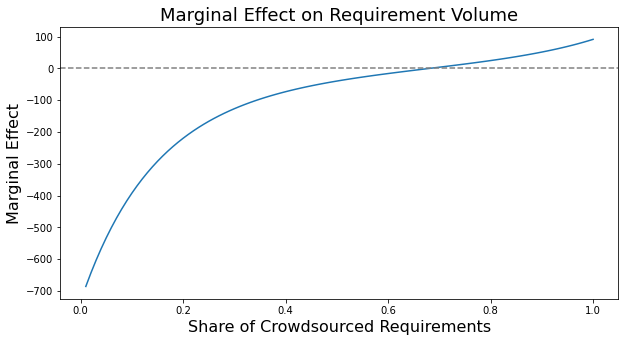
\includegraphics[width=0.85\textwidth]{img/issue_volume_marginal.PNG}
\caption{Marginal effects on issue volume as a function of crowdsourcing.}
\label{issue_volume_marginal}
\end{figure*}

As noted in Section \ref{measures_of_effectiveness}, an increase in requirement volume can represent a positive or a negative outcome, depending on the circumstances. Project managers can determine the costs and benefits of an increase in requirement volume by plotting the trade-off space between requirement volume and other measures of effectiveness. Figure \ref{leaflet_trade_space} shows the trade-off analysis for LeafletJS, a JavaScript geospatial library. In this example, an increase in requirement volume results in longer response and close-out times and less comment activity on each requirement, reflecting a trade-off between levels of crowd engagement and the comprehensiveness of the requirement set. The trade-off plots suggest the presence of two phenomena. First, growing crowd sizes result in social loafing, whereby crowd members comment less actively on requirements in the expectation that other members of the crowd will pick up the slack. Second, the increase in close-out time may reflect the need to validate and clarify more complex uses cases, which arise due to feedback from a more diverse set of stakeholders. In addition to requirements elicitation, these trade-offs imply that project managers should engage with the crowd to validate and prioritize requirements. Collaborative requirements elicitation techniques~\cite{stakerare, mobasher} can aid in that endeavor. At certain levels of engagement, projects may benefit more from validating existing requirements than from sourcing new ones. Trade-off plots provide project managers with the ability to make an informed decision based on the circumstances specific to a project.

\begin{figure*}
  \includegraphics[width=0.95\textwidth]{img/leaflet_trade_space.png}
\caption{Trade-off space as requirement volume increases for LeafletJS.}
\label{leaflet_trade_space}
\end{figure*}